\documentclass[12pt]{article}
 
\usepackage[utf8]{inputenc}
\usepackage[T1]{fontenc}
\usepackage{lmodern}
\usepackage[ngerman]{babel}
%%\usepackage{geometry}
%%\geometry{a4paper}

\usepackage{amsmath}
\usepackage[pdfborder={0 0 0}]{hyperref}
\usepackage{graphicx}
\usepackage{setspace}
\onehalfspacing


\begin{document}
 
%deckblatt start
\thispagestyle{empty}
\begin{center}
\Large{Technische Universität Dresden}\\
\end{center}
 
 
\begin{center}
\Large{Fakultät Informatik}
\end{center}
\begin{verbatim}
 
 
\end{verbatim}
\begin{center}
\textbf{\LARGE{Praktikumsbericht}}
\end{center}
\begin{verbatim}
 
 
\end{verbatim}
\begin{center}
\textbf{im Diplomstudiengang Informatik}
\end{center}
\begin{verbatim}
 
 
\end{verbatim}
 
\begin{flushleft}
\begin{tabular}{lll}

& & \\
& & \\
& & \\
& & \\
& & \\
\textbf{eingereicht von:} & & Josef Schulz \\
Matrikel-Nr. & & 3658867 \\
& & \\
\textbf{eingereicht am:} & & 20. März 2014\\
& & \\
& & \\
\textbf{Betreuer:} & & Prof. Dr. Uwe Aßmann
\end{tabular}
\end{flushleft}
 
%deckblatt ende

\newpage

\tableofcontents

\newpage

\section{Vorbetrachtung}

\subsection{Begebenheiten}

Die Leidenschaft zur Informatik habe ich bei meinen ersten Programmierversuchen in der Schulzeit entwickelt.
In den folgenden Jahren begann ich meine Kenntnisse zu vertiefen und meine Fähigkeiten in Theorie
und Praxis weiter zu verbessern. Das Studium der Informatik an der TU Dresden bietet die Möglichkeit,
ein 20-wöchiges Praktikum zu absolvieren oder ein Semester im Ausland zu studieren.

Einige meiner Professoren bemängelten während der Vorlesungen die ungenügende praktische Erfahrung von
Absolventen. Zudem zeigte sich mir in den vergangenen Semestern, wie viel Zeit sich durch ausreichende Übung
bei der Realisierung von Algorithmen einsparen lässt. Im Theoretischen scheint die eigentliche Programmierung
oft als ein trivialer Faktor, der bezüglich des Zeitaufwandes oft unterschätzt wird. 
Ein nicht seltenes Problem, welches zu verspäteten Veröffentlichungen führt.
So bleibt nach Aussage eines Professors oft keine Zeit, mit Parametern zu experimentieren.
Optimale Ergebnisse werden deshalb nur selten erreicht.
Ein Praktikum motiviert zum Sammeln von Erfahrungen in praxisorientierten Anwendungsbereichen. Damit sind sowohl
theoretische und praktische Erfahrungen im Bereich der Programmierung und Modellierung gemeint.

Eine gute Möglichkeit für Praktika bieten meiner Meinung nach insbesondere kleinere Unternehmen. 
Kleine Betriebe beschäftigen wenige Mitarbeiter die Arbeiten in unterschiedlichen Bereichen umsetzen müssen.
Ein Praktikant bekommt demnach die Möglichkeit, viele Facetten in einem oder mehreren Projekten kennenzulernen.
Die Einbeziehung in den Entwicklungsprozess ist wesentlich, da die vorhandenen personellen Ressourcen oft knapp
bemessen sind.
 
Ein wichtiger Faktor, der mich zur Absolvierung eines Praktikums angeregt hat, war das Interesse an meinem
eigenen Entwicklungsstand. Durch die Mitarbeit in einem Unternehmen bekommt man es mit praktischen Problemen
zu tun, die es zu lösen gilt.

Im Folgenden möchte ich auf meine Motivation und Erwartungshaltung vor dem Praktikumsbeginn eingehen.

\subsection{Nutzen des Praktikums}

Jeder Informatikstudent an der TU Dresden absolviert im dritten Semester, in Form einer Gruppenarbeit, das Softwaretechnologiepraktikum.
Für nicht wenige ist dieses das erste Projekt, in dem sie gemeinsam mit anderen ein Ziel erreichen müssen. 
Auf Grund der Größe dieses Projektes benötigt ein solches Programm eine gute Struktur, die nur durch eine
gute Kommunikation und Organisation der Gruppe eingehalten werden kann.

Die Arbeit aus dem dritten Semester umfasste bei meiner Gruppe in etwa 8000 Zeilen Quelltext. 
Unsere Projektarbeit war nur ein Anfang. Zu einer Version, die verkauft werden könnte, steckten noch zu viele Unzulänglichkeiten
im Detail.
Projekte, die von Betrieben vorangetrieben werden, sind oftmals ein Vielfaches größer als jene, die ein
Informatikstudent während seiner Ausbildung im Allgemeinen zu sehen bekommt.
Es erfordert Übung und Disziplin, die nötige Struktur zu wahren und dadurch den Überblick behalten zu können.
Das Praktikum sehe ich als Basis, um mich in den bereits angesprochenen Fähigkeiten zu üben.

Zur Absolvierung meines Berufspraktikums habe ich die \href{https://alaun.de/home/}{alaun GmbH} gewählt.
Bevor ich die Firma \href{https://alaun.de/home/}{alaun GmbH} und meinen Aufgabenbereich in dieser erläutere,
 möchte ich einen kurzen Abriss über meine Vertiefungen aus meinem Hauptstudium geben. 
Mein Hauptaugenmerk liegt im Bereich der Grafikprogrammierung, der Bildverarbeitung und insbesondere im Gebiet des Maschinellen Lernens.
Bei den Programmierarbeiten in diesen Fachrichtungen geht es um Effizienz und Geschwindigkeit, zu Gunsten dieser wird auf
\textit{Design Pattern} und ähnliche Techniken verzichtet. Diese Modelle sind oft unerlässlich, wenn es um die
Entwicklung und Verteilung von großen Projekten geht.
Mit dem Bereich der Softwaretechnologie hatte ich mich zu diesem Zeitpunkt nur im Rahmen meines Grundstudiums beschäftigt. 
Mit Webentwicklung hatte ich nur am Rande durch das Softwaretechnologiepraktikum im dritten Semester zu tun gehabt.
Der Anteil an Erfahrungen, die ich insbesondere in diesem Gebiet gesammelt hatte, war eher gering.
Um welche Schwerpunkte es in meiner Zeit in der \href{https://alaun.de/home/}{alaun GmbH} gehen sollte, war mir bis zum
Beginn des Praktikums nur wenig bekannt.

\subsection{Formalitäten}

Der für das Praktikum beanschlagte Zeitraum beträgt 20 Wochen. Diese habe ich vom 1. September 2013
bis zum 31. Januar 2014 in der \href{https://alaun.de/home/}{alaun GmbH} absolviert.

\section{alaun GmbH}

\subsection{Impressum}

\begin{minipage}{\linewidth}

alaun GmbH \\
Hoyerswerdaer Straße 20 \\
01099 Dresden \\

Tel (0351) 563406-0  \\
Fax (0351) 563406-29 \\

mail@alaun.de 

\end{minipage}

\subsection{Übersicht}

Bei der \href{https://alaun.de/home/}{alaun GmbH} handelt es sich um ein Unternehmen mit Sitz in Dresden.
Die \href{https://alaun.de/home/}{alaun GmbH} beschäftigt 11 Mitarbeiter, die auf zwei Hauptprojekte verteilt
sind. Das erste, Business ByDesign, soll hier nur aus Gründen der Vollständigkeit erwähnt werden, 
da ich an diesem Projekt nicht beteiligt war. Das zweite trägt firmenintern den Titel \textit{Eine neue Welt}.
Hierbei handelt es sich um einen Arbeitsbegriff für zwei Content Management Systeme, die im Folgenden mit CMS abgekürzt werden.

\subsection{Hauptprojekte}

\subsubsection{Business ByDesign}

Unter dem Namen Business ByDesign werden Anwendungen und Komplettlösungen anderer Unternehmen für den
Endkunden angepasst. So zum Beispiel eine SAP Software, die bei einer in Dresden ansässigen Brauerei zum Einsatz kommt.

\subsubsection{Eine neue Welt}

Im Jahr 2001 begann deutschlandweit der Verkauf des CMS-Tools Elexir an die Sparkasseninstitutionen. 
Mit diesem Tool werden die Internetauftritte der einzelnen Institute gestaltet. 
Besonders hervorzuheben ist die Größenordnung und die Anzahl der zu verwaltenden Projekte. Jedes Institut gestaltet im Prinzip unabhängig von den anderen seine Onlinepräsenz.
Gänzlich voneinander zu trennen sind diese allerdings auch nicht, da Werbung, Kundeninformationen und Designs in
Regionen-basierten Hierarchien vorgegeben und geteilt werden.

Nach 13 Jahren Laufzeit hat die \href{https://alaun.de/home/}{alaun GmbH} mit einer Neuauflage des Projektes begonnen.
Mit einem sprach-basierten Ansatz wird Problemen begegnet, die durch verteilte Entwicklung in dieser Größenordnung
entstehen. Namen und Ids werden automatisch generiert und vor dem Benutzer verborgen. 
Die entwickelte Sprache trägt den Namen Cauldron und wird durch ein Java-Backend realisiert.
Cauldron ist eine XML-basierte Sprache und dient zur Entwicklung von Internetseiten.
Im Gegensatz zu HTML gibt es eine Vererbungshierarchie. Durch diese wird Redundanz beim Programmieren vermieden.
Neben den sogenannten \textit{namespaces} gibt es \textit{Module} und \textit{Fragmente}, durch die sich
Programmkomplexe kapseln und überlagern können. 


\section{Verlauf}

\subsection{Der erste Arbeitstag}

Am 2. September 2013 um 09:00 Uhr begann für mich die Zeit in der \href{https://alaun.de/home/}{alaun GmbH}.
Zu Beginn lernte ich die Firma kennen und die bereits oben erwähnten Projekte wurden mir erläutert.
Da die \textit{neue Welt} zu diesem Zeitpunkt eines besonderen Entwicklungsaufwandes bedurfte, entschied ich mich,
an diesen Projekt aktiv teilzunehmen.

Um mich mit der Thematik vertraut zu machen, las ich das Pflichtenheft und sämtliche Dokumente, welche die Firma
zu diesem Projekt verfasst hat. 

\subsection{Entwicklungsumgebung und Technologien}

Nach der grundlegenden Einarbeitung begann ich, die Entwicklungsumgebung einzurichten und mich in Technologien
wie zum Beispiel Maven und OSGI einzuarbeiten. Die \href{https://alaun.de/home/}{alaun GmbH} hat für die Korrektur
des Cauldron-Quelltextes ein eigenes Plugin bereitgestellt, durch welches die Entwicklung eigener Cauldron-basierter
Projekte erleichtert wird. Interpretiert wird der Cauldron-Quelltext durch ein Java-Servlet. 
Da für die Einrichtung der Entwicklungsumgebung noch keine Dokumente existierten, dokumentierte ich meine Schritte,
um nachfolgenden Programmierern einen schnelleren Einstieg in das Projekt zu ermöglichen.

Meine Kenntnisse auf dem Gebiet der Web-Programmierung ließen noch zu wünschen übrig, weshalb ich mit der Entwicklung
eines primitiven Funktionsplotters begann. Ziel der Übung war es, mich mit Cauldron erst einmal vertraut zu machen.
Ich bekam Unterstützung von einem versierten Kollegen, der mir nicht nur programmiertechnische Aspekte der Web-Entwicklung näher bringen konnte.
Farben und Aufteilungen waren ebenfalls Bestandteil meines Trainings. 
Zum Zeichnen der Funktionen diente ein Canvas Element und Javascript.
Nach der Fertigstellung des Funktions-Plotters für einen normalen Browser konnte ich mit den Methoden von Cauldron
binnen kürzester Zeit eine Mobile Version der Seite fertig stellen.
Hier zeigten sich die Vorzüge von Komponenten und Vererbungen, mit deren Hilfe die Anzahl an Quelltextzeilen gering gehalten
werden konnte.

\subsection{Entwicklung von Komponenten}

Entwickelt man ein CMS-System, sind einfache Komponenten wie Textfelder und Bezeichner, welche von HTML bereitgestellt werden,
nur ein Anfang. Im Folgenden begann ich bei der Entwicklung der Komponenten zu helfen. Als Beispiel dient eine einfache Textbox
mit Bezeichner. Eine solche Komponente bringt mehrere Variablen mit sich. Damit ist zum einen der Inhalt des Bezeichners und der
voreingestellte Inhalt der Textbox gemeint, zum anderen werden auch die Möglichkeiten zum Gestalten und Platzieren vorgegeben.
Auf diese Weise können sehr komplexe Komponenten entstehen und es lässt sich eine breite Palette an Bankformularen konzipieren.

Cauldron bietet aber noch viel mehr als Designs und Formulare. Der Workflow ist eine backendbasierte Realisierung eines 
Mealyautomaten. Durch den Einstatz von Workflows lassen sich funktionale Komponenten konstruieren, die sich im späteren Editor
mit der Maus schnell auf eine Seite ziehen lassen.

Eine Komponente ist eine Art Container, mit der Möglichkeit, Parameter zu übergeben und den Einsatz möglichst variabel zu gestalten.
Komponenten können von anderen Komponenten erben und haben eine gewisse Ähnlichkeit mit Klassen. Daher eignet sich UML sehr gut zur
Modellierung von Komponentenstrukturen.

\begin{figure}[h]
	\centering
	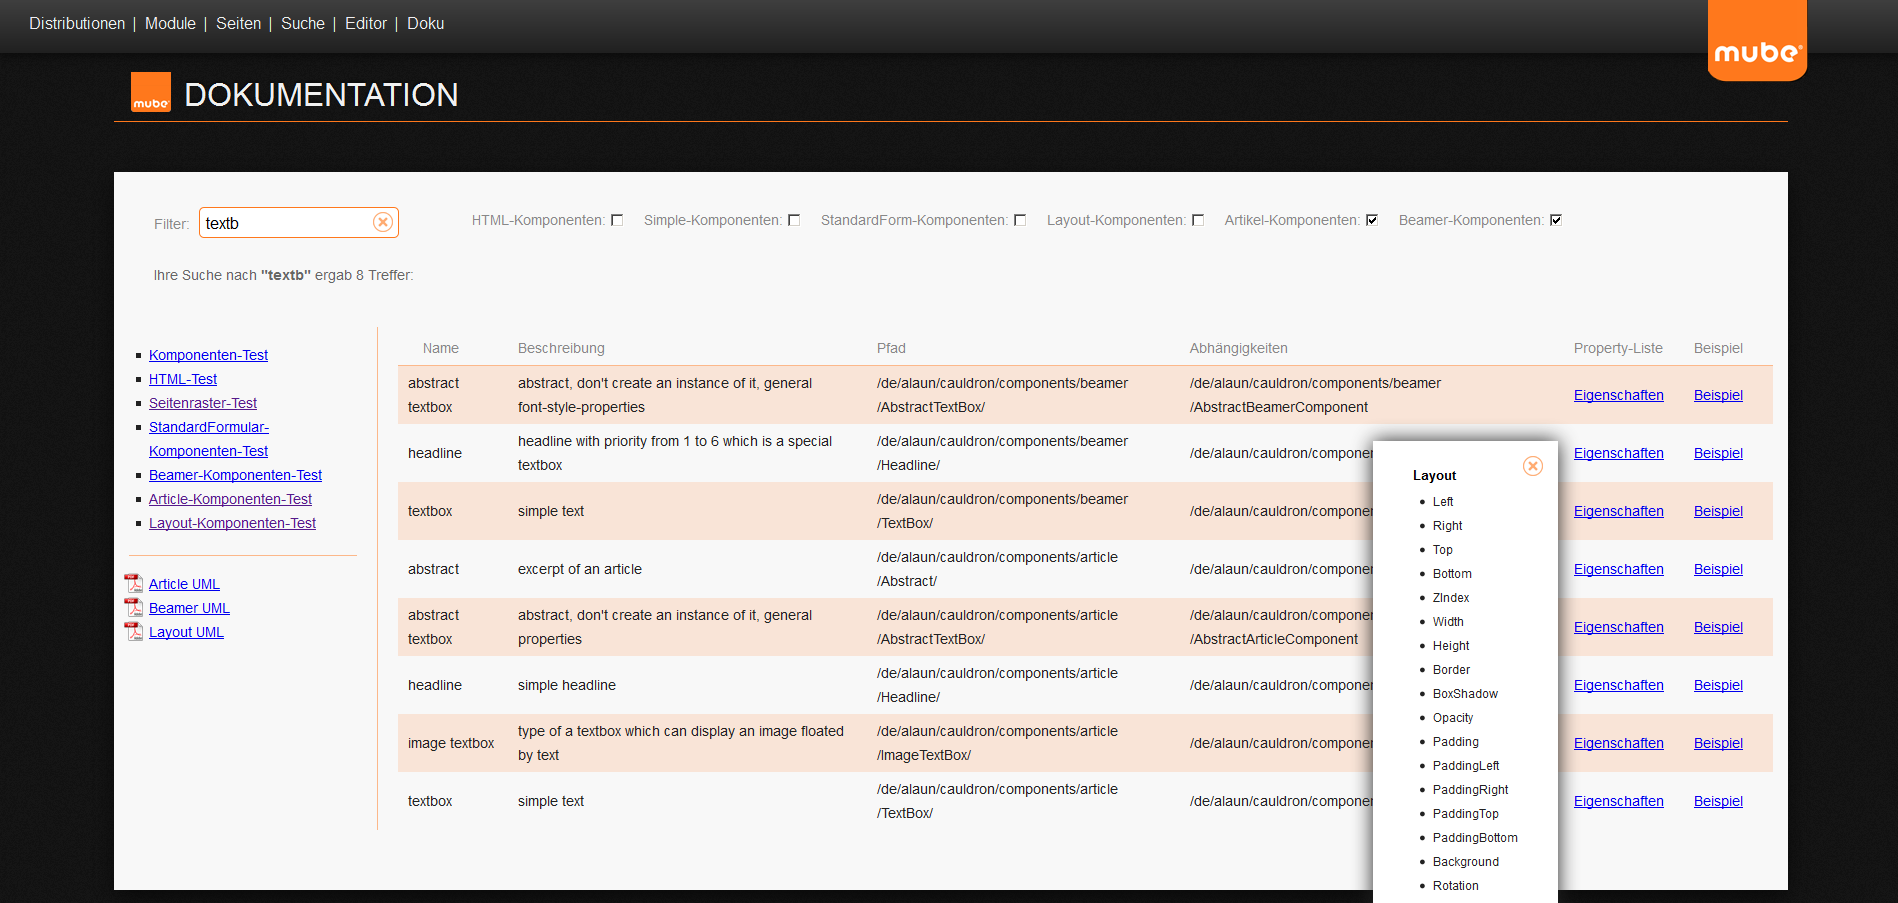
\includegraphics[width=1.0\textwidth]{DokuPage.png}
	\caption{Komponenten Dokumentation}
	\label{fig:DokuPage}
\end{figure}

Neben der Entwicklung der Komponenten haben wir eine Dokumentation dieser erstellt. Im Verlauf dieser Entwicklung haben wir
den Prozess der Dokumentierung vereinfacht. Um nicht jedes mal an mehreren Stellen bei Änderungen die Einträge bearbeiten zu müssen,
führten wir Tags ein. Mögliche Variablenbelegungen wurden automatisch aus den Komponenten generiert. Ein Ausschnitt der Dokumentation
wird in der Abbildung \ref{fig:DokuPage} dargeboten.

\subsection{Seitenlayouts}

\begin{figure}[h]
	\centering
	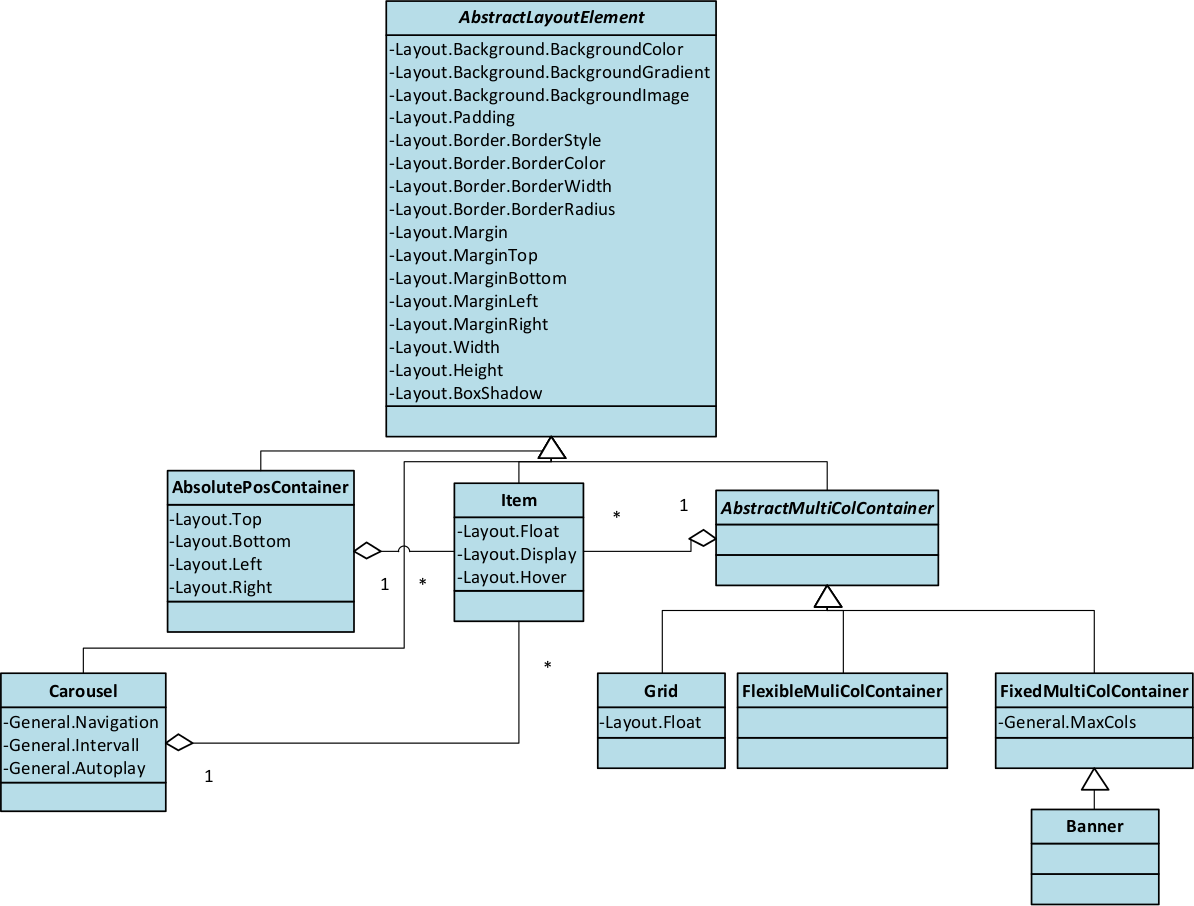
\includegraphics[width=1.0\textwidth]{Layout.png}
	\caption{Layout-Komponenten UML-Diagramm}
	\label{fig:Layout}
\end{figure}

Ein weiteres Aufgabenfeld bestand in der Entwicklung von Komponenten für standardisierte Seitenformen, wie den Artikel und
eine Präsentations-Komponente. In beiden Fällen haben wir bestehende Programme studiert und daraus Komponenten-Strukturen
mit UML-Diagrammen abgeleitet und ergänzt. Die Abbildung \ref{fig:Layout} zeigt die Komponenten Struktur für unsere Layout-Container, mit deren
Hilfe sich Inhalte automatisch anordnen lassen.

\subsubsection{Präsentations-Komponenten}

\begin{figure}[h]
	\centering
	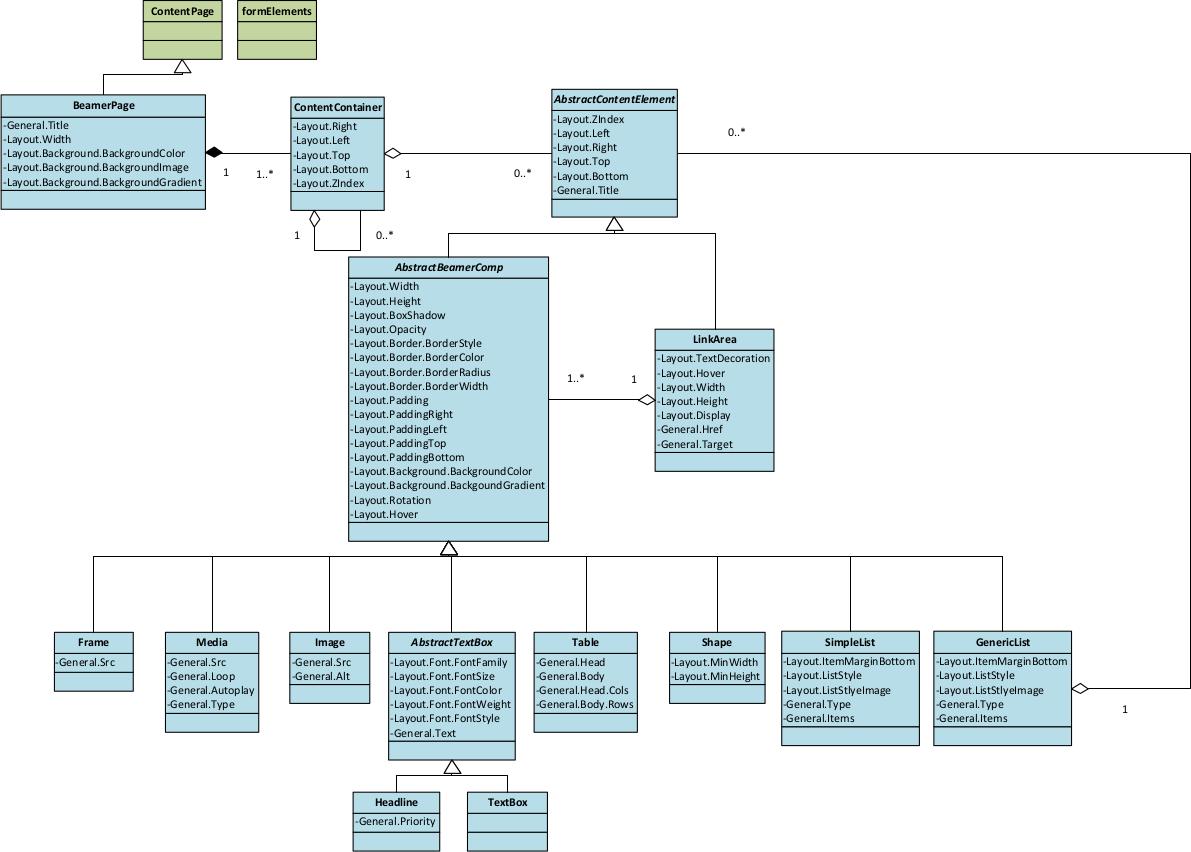
\includegraphics[width=1.0\textwidth]{Beamer.png}
	\caption{Präsentations-Komponenten UML-Diagramm}
	\label{fig:Beamer}
\end{figure}

Die Präsentationsseite besteht aus mindestens einem Container für Inhalt, diese können entweder aus Containern oder aus Elementen bestehen.
Es gibt eine Vielzahl von Elementen, die sich innerhalb eines Containers absolut positionieren lassen. Die Abbildung \ref{fig:Beamer} zeigt
das UML-Diagramm, das die Komponenten Struktur unserer Präsentations-Komponenten widerspiegelt. 

Um einen kurzen Einblick in die Funktionsweise unserer Präsentations-Komponenten zu geben, möchte ich auf die \textit{LinkArea} etwas genauer eingehen. 
Die grundlegenden Elemente, die in einem Container platziert werden können, werden als \textit{AbstractContentElement} bezeichnet. Von diesem leitet sich auf der einen Seite die \textit{AbstsractBeamerComp} und auf der anderen Seite die \textit{LinkArea} ab. 
Letztere besteht ebenfalls aus Elementen des Typs \textit{AbstsractBeamerComp}. 
In einer \textit{LinkArea} enthaltene Elemente dienen zur Gestaltung des Links. Farben und Formen
können überschrieben werden, wodurch sich zum Beispiel Farben beim sogenannten Hovereffekt verändern lassen.

\subsubsection{Artikel-Komponenten}

\begin{figure}[h]
	\centering
	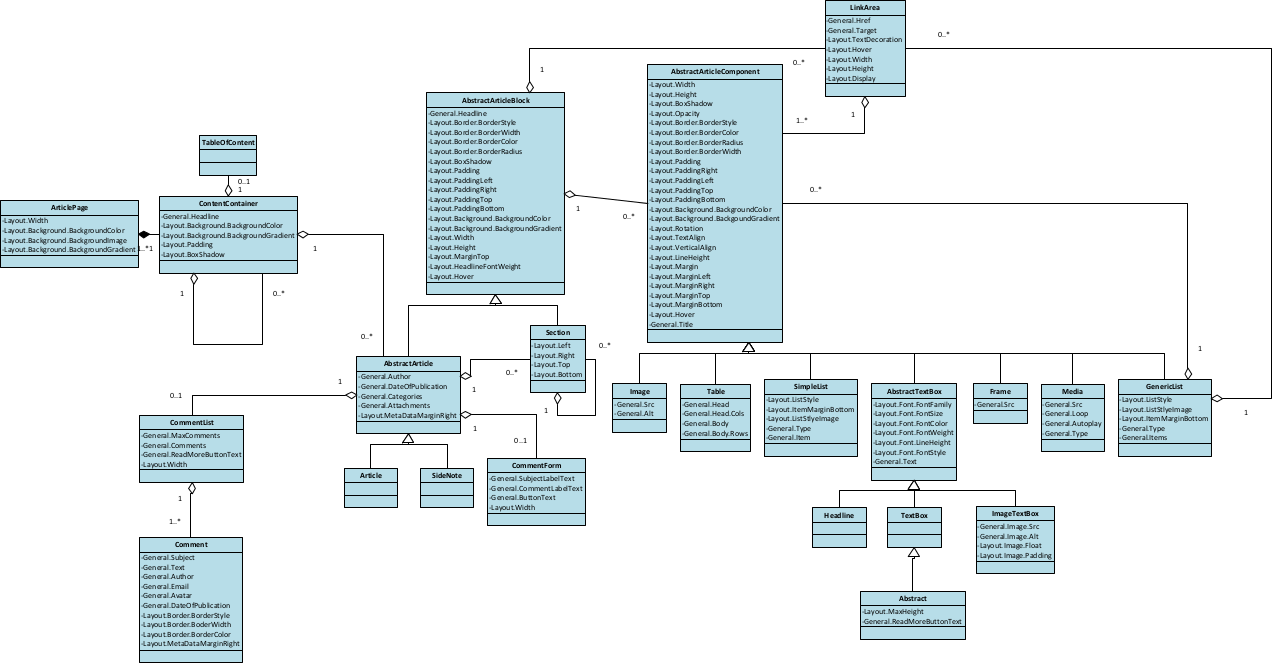
\includegraphics[width=1.0\textwidth]{Artikel.png}
	\caption{Artikel-komponenten UML-Diagramm}
	\label{fig:Artikel}
\end{figure}

Die Artikel-Komponenten bilden einen weiteren Seitentyp der aus einer Vielzahl von bestehenden Programmen
bekannt sein dürfte. In der Abbildung \ref{fig:Artikel} ist das entsprechende UML-Diagramm dargeboten.
Der prinzipielle Aufbau erinnert an die Präsentations-Komponenten, er unterscheidet sich hinsichtlich
der Positionierungen und Unterteilungen. Ist eine Präsentation auf eine bestimmte Seitengröße festgelegt, ist diese bei der Artikelseite
nicht vorgegeben. Artikel können beliebig lange Seitenverläufe formen, sich aber auch in kleinere Seiteneinheiten unterteilen lassen.
Direkt integriert ist in Anlehnung an diverse Blogs eine Kommentarliste mit dem entsprechenden Formular zum Hinterlassen
von Kommentaren entstanden.

\subsection{Entwicklung mit WebGl}

Nach der Entwicklung dieser Komponentenstrukturen hatte ich die nötige Zeit, um mich mit WebGl zu beschäftigen. Durch WebGl ist es möglich,
komplexe Szenen direkt im Browser darzustellen und die Grafikkarte zur Berechnung der Szene mit einzubeziehen.
Zur Gestaltung der Seitenkomponenten, welche nicht durch WebGL gerendert wurden, wie \textit{Buttons}
und \textit{Checkboxen}, benutzte ich HTML und CSS ohne Cauldron. Dabei zeigten sich die Vorzüge Cauldrons besonders deutlich.
Der Unterschied war um so gravierender, je mehr identische Objekte auf einer Seite benötigt wurden. Diese Erfahrung zerstreute den Rest Skepsis,
den ich gegenüber dem Cauldron-Projekt bis zu diesem Zeitpunkt hatte. Durch die Entwicklung mit WebGl lernte ich einiges über Javascript,
insbesondere was die Effizienz verschiedener Implementierungen angeht. Der Einsatz von WebGl könnte ebenso für besondere Darstellungsvarianten
in das CMS integriert werden. Als Beispiel könnte die Animation eines Sparkassensymbols dienen. Im Gegensatz zu einfachen Gifs wäre es interaktiv
und bietet nahezu unbegrenzte Möglichkeiten, in Bezug auf Gestaltung. Der Einsatz auf mobilen Geräten ist auf Grund der benötigten Rechenleistung eher ein
Zukunftstraum. Eine interessante Möglichkeit würde sich durch das Rendern von HTML in Texturen ergeben. Durch den Einsatz von Techniken wie WebGl sind beliebige Animationen in einem dreidimensionalen Raum in Echtzeit erzeugbar. 
Eingabegeräte könnten ebenfalls in den 3D-Raum abgebildet werden, was zu interessanten Bedienungsformen führt.
So ließen sich Inhalte, zum Beispiel auf die Seiten in einem Buch, mit HTML erstellen. Die Seiten des Buches könnten im Anschluss
beliebig durchgeblättert werden und trotzdem in jeder Position interaktiv sein.

\subsection{Entwicklung eines Addon-Managers für Elexir}

Neben dem bisher behandelten Neubau eines CMS-Tools pflegt die \href{https://alaun.de/home/}{alaun GmbH} den Vorgänger mit dem Namen Elexir.
Updates und Neuerungen werden nach wie vor für Elexir geliefert. 
Die Struktur von Elexir erlaubt es ebenfalls, mit einer XML-basierten Sprache Anpassungen vorzunehmen. 
Die \href{https://alaun.de/home/}{alaun GmbH} stellt externen Firmen Werkzeuge zur Entwicklung für derartige
Erweiterungen bereit. Um diese Erweiterungen in Elexir einspielen zu können, haben wir einen Addon-Manager entwickelt. 
Dieses Tool besteht ebenfalls aus einer Reihe von Scripts und ermöglicht die Anbindung an einen Händler für derartige Addons.

Bisher wurden Erweiterungen und Neuerungen zu bestimmten Release-Zeitpunkten in Form von gepackten Archiven händisch von den Administratoren in Elexir eingespielt. 
Mit der Lieferung des Addon-Managers ist diese Vorgehensweise nur noch ein letztes Mal nötig.

Die Addons von externen Firmen werden als verschlüsselte Version mittels Git von den alaun-Servern angezogen. Bevor diese als Neuerscheinung oder als Update bei dem Onlinehändler erscheinen, werden die Addons von einem Programm auf Vollständigkeit überprüft und entsprechend freigeschaltet oder zurückgehalten. 

\begin{figure}[h]
	\centering
	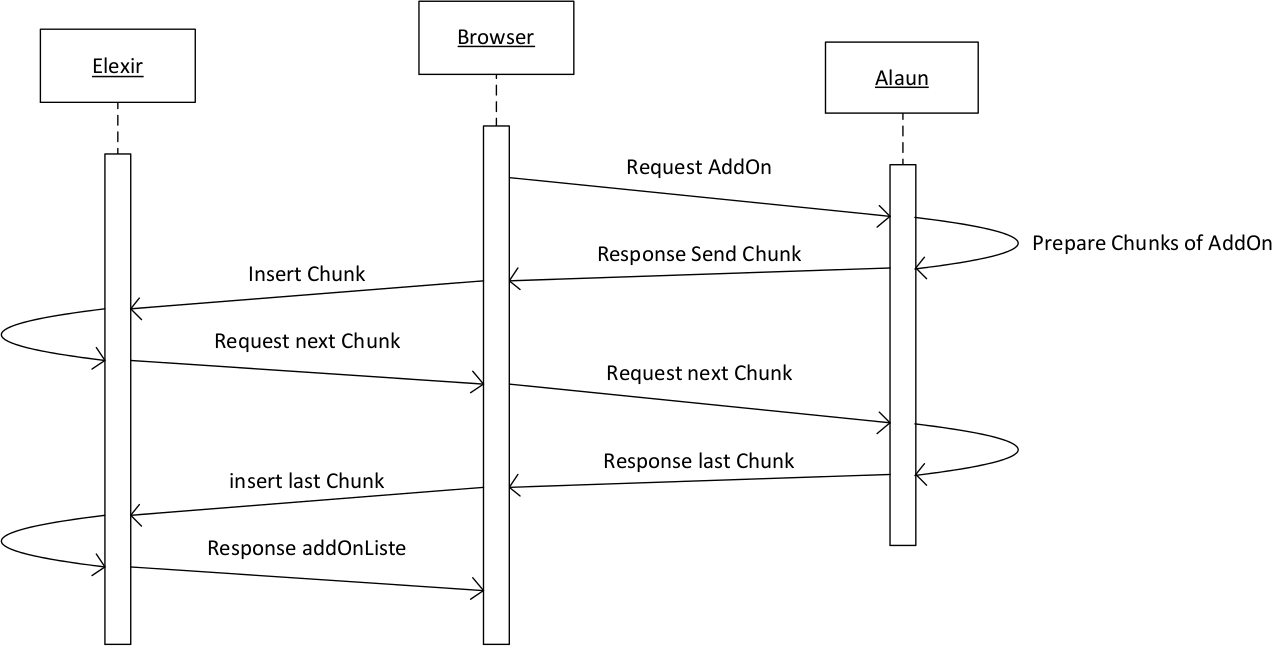
\includegraphics[width=1.0\textwidth]{Manager.png}
	\caption{Download Squenzdiagramm}
	\label{fig:Manager}
\end{figure}


Der Addon-Manager löst die Kommunikation zwischen dem entsprechenden Elexir-Client und den alaun-Servern. Ein Elexir-Client kann nicht direkt mit den alaun-Servern kommunizieren, da beide über eine \textit{HTTPS} Verbindung laufen. Als Schnittstelle dient der Browser des Elexir-Nutzers.
Die Kommunikation ist Beispielhaft in Abbildung \ref{fig:Manager} dargestellt. 

Beim Zugriff auf den Addon-Manager wird ein \textit{JSONP-Request} ausgeführt mit dessen Hilfe eine Liste mit Addon-Id und Version an die alaun-Server gesendet wird. 
Der nächste Schritt besteht aus einer Prüfung der Aktualität. Die alaun-Server vergleichen die Addon-Versionen und setzt gegebenenfalls ein Flag. 
Die Liste an aktualisierbaren Addons wird dem Browser jetzt als Parameter der Response-Funktion übergeben.

Im Folgenden wird dem Nutzer eine Liste mit seinen Addons angezeigt. Wurde das Flag für \textit{update} gesetzt, wird ein Button erstellt.
Mit Hilfe dieses Buttons kann das spezifische Addon aktualisiert werden. Weiterhin besteht die Möglichkeit alle Addons in einem Schritt zu aktualisieren.
Neue Addons können über den \textit{Addon-Store} erworben werden. Dazu wird über den Browser ein Button als Link angeboten, über diesem gelangt der Nutzer zu einer Liste Installierbaren Addons.
Dargeboten werden jene Addons, für die der Nutzer noch keine gültige Lizenz erworben hat.

Die Methode zum Installieren oder zum Aktualisieren ist sehr ähnlich aufgebaut. Es wird ein Request über den Browser an die alaun- Server gesendet, Addon-Name
und gewünschte Version werden übergeben. Ob es sich um ein Update oder eine Neuinstallation handelt wird ebenfalls mittels Flag mitgeteilt.
Dieser Request geht an ein Servlet der alaun-Server. Das Servlet baut das geforderte Addon zusammen und erstellt ein Archiv,
in Form einer Zip-Datei. Danach wird
der \textit{Bytestream} in einzelne Chunks unterteilt und verschlüsselt. Die Chunks werden sukzessiv über ein Formular gesendet. Die Seite mit dem Formular welche vom Browser gerendert wird, führt eine Weiterleitung zu Elexir durch und übergibt den Chunk an Elexir.

Meine Aufgabe bestand in der Entwicklung des Servlets, welche die Zip-Dateien aus den Addons erstellt, zerlegt und Chunk für Chunk über das Formular durch den Browser an Elexir sendet.
Nachdem die Grundfunktionalität bereit gestellt wurde habe ich mich um die Anbindung einer Datenbank gekümmert. Mit der Datenbank wird sichergestellt,
das kein Kunde Testversionen mehrmals Nutzen kann. Abgeschlossene Kaufverträge werden ebenfalls durch diese Datenbank verwaltet und werden zur
Lizenzgenerierung benötigt.

Nach dem der Prototyp einwandfrei seine Arbeit verrichtet hat, wurde fieberhaft an der Reduzierung der zu Übertragenden Daten gearbeitet.
Wenn Addons aktualisiert werden, dann wurden im Prototyp die Alten Addon-Daten mit denen aus der Neuen Version einfach überschrieben. 
Es ist ein weiterer Schritt zur Bestimmung der Unterschiede zwischen den Versionen hinzugekommen. Auf diese Weise werden nur die Fehlenden Informationen gesendet. Dadurch wird nur noch ein Minimum an Daten übertragen. Durch dieses Vorgehen
lässt sich ein Addon besser Personalisieren. Abweichungen von dem Standard Addon werden durch die Software erkannt.

\subsection{Umstellung des Webauftrittes}

Meine Aufgabe am Addon-Manager war zu diesem Zeitpunkt weitgehend beendet. Meine neue Aufgabe bestand darin in Zusammenarbeit mit einem Kollegen
die Internet-Seite von der \href{https://alaun.de/home/}{alaun GmbH} mit Cauldron neu aufzusetzen und auf dieser die Alaun-eigenen Produkte und Addons Modern zu repräsentieren.
Die Aufgabe bestand nicht nur in der Gestaltung und Beschreibung der \href{https://alaun.de/home/}{alaun GmbH} auf ihren Internetauftritt.
Darüber hinaus galt es den Server einzurichten, die nötigen Programme zu installieren und das Cauldron Projekt zu kompilieren.
Zur Bewerkstelligung dieser Aufgabe haben wir ein \textit{Apache} installiert. Das Projekt haben wir mit Maven kompiliert.
In meiner Einleitung habe ich erwähnt, dass die Realisierung oft einige Probleme mit sich bringt.
So ließ sich das Projekt erst nach einigen Anläufen kompilieren, als Problem erwiesen sich Parameter der Sprache Java.
Erst nach der Anpassung an das Projekt gelang die Ausführung unseres Programms. Die Behebung dieser Fehler benötigte eine
Menge Zeit. 

Nach dem das Projekt in unserem lokalen Netz verfügbar war, erstellten wir Testfälle und versuchten Fehler zu provozieren so weit dies möglich war.
Schwerwiegende Probleme blieben aus, kleinere verwaiste Links fanden wir ab und an. Mit Hilfe von \textit{Selenium} und \textit{JUnit} lassen sich
Testverfahren automatisieren und Internetseiten auf Vollständigkeit überprüfen. Zusätzlich wurde ein Forum eingerichtet um Support anbieten zu können.


\subsection{alaun geht online}

Nach Abschluss der Arbeiten und dem erfolgreichem Absolvieren der Tests und nachdem die nötigen Zertifikate ausgestellt waren,
feierten wir die Veröffentlichung der neuen Internetseite zusammen mit der Veröffentlichung unseres Addon-Managers.
In welchem Rahmen diese Möglichkeiten genutzt werden bleibt abzuwarten.

\subsection{OCR als Zukunftsprojekt}

Nachdem die Arbeiten an dem Addon-Manager und der Internetseite abgeschlossen waren, wurde mir eine neue Aufgabe aufgetragen.
Die Aufgabe besteht in der Entwicklung einer Software, die Informationen für Banküberweisungen erkennt und in
entsprechende Formularfelder einträgt.
Der Schwerpunkt der Aufgabe liegt in der Algorithmik. Das Problem unterteilt sich in mehrere Teilprobleme.
Als Erstes muss das Bild mit den nötigen Informationen gegebenenfalls entrauscht und zur weiteren Verarbeitung
aufbereitet werden. Im zweiten Schritt müssen die Wörter, Buchstaben und Zeichen erkannt werden. Der dritte
Schritt befasst sich mit der Klassifizierung der einzelnen Wörter.
Dazu wird im Text nach Schlüsselwörtern gesucht.
Ausgehend von den Positionen dieser auf dem Blatt Papier werden die zugehörigen Werte bestimmt.
Dazu kann Vorwissen verwendet werden. Es gibt bei BIC und IBAN bestimmte Bildungsvorschriften und Größenordnungen.
Wurden diese Positionen ebenfalls gefunden, werden die ungewissen Felder im Text geschätzt.
In Schritt 4 werden die Daten in ein Formular geschrieben. Jetzt hat der Anwender die Möglichkeit, Fehler, die bei der Erkennung
aufgetreten sind, zu korrigieren.

\subsubsection{OCR als Teilproblem}

OCR steht für \textit{optical charakter recognition} und bezeichnet das Erkennen von Zeichen in Bildern.
Zu Beginn bestand der Anspruch im Finden einer guten OCR Software und der Portierung dieser.
Es stellte sich heraus, dass die meisten OCR-Systeme schnell an ihre Grenzen kamen. 
Unter den freien Programmen wie \href{http://code.google.com/p/tesseract-ocr/}{\textit{Tesseract}} und \href{http://code.google.com/p/ocropus/}{\textit{OCRopus}} fanden sich keine Exemplare, deren Erkennungsfähigkeiten
auch nur im Entferntesten an die benötigten Erkennungsraten herankamen.
Die Implementierung von Acrobat Text Capture hat als einzige getestete Software ein akzeptables Ergebnis erzielt.

Ohne ein gutes OCR-System lässt sich das Problem jedoch nicht lösen. Ich habe innerhalb von einer Woche ein primitives
einfaches OCR-System implementiert. Dieses zerlegt das Problem in zwei Teilprobleme. Als Erstes werden die Buchstaben
einzeln segmentiert. Ein vielversprechendes Verfahren ist hierbei das der \textit{Maximalen Stabilen Regionen}. 
Die segmentierten Buchstaben wurden in kleine Bilder mit 64x64 Pixeln mit 8 Bit Farbtiefe transformiert.
Diese kleinen Bilder von den Buchstaben werden im Anschluss mit Hilfe eines \textit{Feedforward} Netzwerkes klassifiziert.
Die Wortzuordnung erfolgte über die Position der gefundenen Segmente.

Zum Lernen der Klassifikationsfunktion, habe ich ein Reihe von Lernbeispielen verwendet. Diese stammen allerdings nicht
aus einer Datenbank, sondern wurden von mir mittels der Segmentierungsfunktion händisch erstellt. Hier zeigten sich
die ersten Probleme dieses Verfahrens. Nicht bei jedem Text ließen sich die Buchstaben eindeutig segmentieren. Unter
Umständen wurden ganze Wörter als einzelner Buchstabe erkannt. Ein anderes Problem waren Buchstaben wie \textit{i}
und \textit{j}. Aufgrund der Punkte, die zu eben jenen Zeichen gehören, wurden durch den Segmentierungsansatz zum Teil Buchstaben
hinzugefügt. Zu meiner eigenen Freude hat es bei ein paar wenigen Beispielen recht gut funktioniert.

\section{Fazit}

In diesem Fazit möchte ich das Erlebte noch einmal Revue passieren lassen und meine persönliche Meinung zu dem Praktikum äußern.

Die Zeit in der \href{https://alaun.de/home/}{alaun GmbH} begann für mich im September 2013. Nach meiner
Ankunft in dieser kleinen Firma habe ich viele mir unbekannte Technologien und 
Arbeitsfelder der Informatik kennen gelernt. Die Arbeiten die ich als Praktikant verrichtet habe, waren ungemein
vielfältig. Zu Beginn der Einarbeitungszeit habe ich unter professioneller Anleitung einen Praxiskurs in der Webentwicklung
genießen dürfen. Später bekam ich tiefere Einsicht in den Interpreter von Cauldron, ein Projekt mit über 250.000 Zeilen
Quelltext. Der Addon-Manager ist das größte Projekt, an dem ich beteiligt war. Schlussendlich wurde das Projekt durch dessen
Veröffentlichung abgeschlossen. Durch die Probleme, die mit der automatisierten Erfassung von Informationen und deren Weiterverarbeitung zusammenhängen, habe ich bereits ein Thema für die Fertigung eines Beleges gefunden.

Das Praktikum hat meine Erwartungen in Bezug auf Programmiererfahrungen und das Kennenlernen von Technologien weit übertroffen.
Auch mit Kommunikations- und mit Projektmanagement-Konzepten wurde ich belohnt. Meine Ausbildung ist noch nicht zu Ende, aber
die vermittelten Unterrichtsinhalte meines Studiums haben mich auf die Praxis durchaus vorbereitet.
Ich sehe mich mehr denn je in der Lage, Probleme zu lösen und an der Entwicklung von praxisorientierten Projekten mitwirken zu können.
In der \href{https://alaun.de/home/}{alaun GmbH} traf ich auf Menschen mit innovativen Ideen und den Kompetenzen, diese
zu verwirklichen.

Jedem, der sich unsicher ist, welche Richtung er einschlagen möchte, kann ich sagen, dass es nicht auf die Thematik ankommt.
Entscheidend ist die Motivation und die Unterstützung des Teams.
Mit dem letzten Satz möchte ich mich bei allen Beteiligten für die erfolgreichen 20 Wochen bedanken.

\newpage

\section{Eidesstattliche Erklärung}

Ich versichere, dass ich den Praktikumsbericht selbständig verfasst habe. Andere als die angegebenen Quellen und Hilfsmittel wurden nicht verwendet.

\vspace*{3cm}

\noindent Datum und Unterschrift

\end{document}

